%%% The main file. It contains definitions of basic parameters and includes all other parts.

%% Settings for single-side (simplex) printing
% Margins: left 40mm, right 25mm, top and bottom 25mm
% (but beware, LaTeX adds 1in implicitly)
\documentclass[12pt,a4paper]{report}
\setlength\textwidth{145mm}
\setlength\textheight{247mm}
\setlength\oddsidemargin{15mm}
\setlength\evensidemargin{15mm}
\setlength\topmargin{0mm}
\setlength\headsep{0mm}
\setlength\headheight{0mm}
% \openright makes the following text appear on a right-hand page
\let\openright=\clearpage

%% Settings for two-sided (duplex) printing
% \documentclass[12pt,a4paper,twoside,openright]{report}
% \setlength\textwidth{145mm}
% \setlength\textheight{247mm}
% \setlength\oddsidemargin{14.2mm}
% \setlength\evensidemargin{0mm}
% \setlength\topmargin{0mm}
% \setlength\headsep{0mm}
% \setlength\headheight{0mm}
% \let\openright=\cleardoublepage

%% Generate PDF/A-2u
\usepackage[a-2u]{pdfx}

%% Character encoding: usually latin2, cp1250 or utf8:
\usepackage[utf8]{inputenc}
\usepackage[T1]{fontenc}

%% Prefer Latin Modern fonts
\usepackage{lmodern}

%% Further useful packages (included in most LaTeX distributions)
\usepackage{amsmath}        % extensions for typesetting of math
\usepackage{amsfonts}       % math fonts
\usepackage{amsthm}         % theorems, definitions, etc.
\usepackage{bbding}         % various symbols (squares, asterisks, scissors, ...)
\usepackage{bm}             % boldface symbols (\bm)
\usepackage{graphicx}       % embedding of pictures
\usepackage{fancyvrb}       % improved verbatim environment
\usepackage{natbib}         % citation style AUTHOR (YEAR), or AUTHOR [NUMBER]
\usepackage[nottoc]{tocbibind} % makes sure that bibliography and the lists
			    % of figures/tables are included in the table
			    % of contents
\usepackage{dcolumn}        % improved alignment of table columns
\usepackage{booktabs}       % improved horizontal lines in tables
\usepackage{paralist}       % improved enumerate and itemize
\usepackage{xcolor}         % typesetting in color
\usepackage{mathrsfs}		% mathscr
\usepackage[h]{esvect}		% vv
\usepackage{makecell}		% makecell

%%% Basic information on the thesis

% Thesis title in English (exactly as in the formal assignment)
\def\ThesisTitle{Magnetic Transport Along Translationally Invariant Obstacles}

% Author of the thesis
\def\ThesisAuthor{Michal Grňo}

% Year when the thesis is submitted
\def\YearSubmitted{2021}

% Name of the department or institute, where the work was officially assigned
% (according to the Organizational Structure of MFF UK in English,
% or a full name of a department outside MFF)
\def\Department{Institute of Theoretical Physics}

% Is it a department (katedra), or an institute (ústav)?
\def\DeptType{institute}

% Thesis supervisor: name, surname and titles
\def\Supervisor{prof. RNDr. Pavel Exner, DrSc.}

% Supervisor's department (again according to Organizational structure of MFF)
\def\SupervisorsDepartment{Institute of Theoretical Physics}

% Study programme and specialization
\def\StudyProgramme{Physics}
\def\StudyBranch{FOF}

% An optional dedication: you can thank whomever you wish (your supervisor,
% consultant, a person who lent the software, etc.)
\def\Dedication{%
Dedication.
}

% Abstract (recommended length around 80-200 words; this is not a copy of your thesis assignment!)
\def\Abstract{%
Abstract.
}

% 3 to 5 keywords (recommended), each enclosed in curly braces
\def\Keywords{%
{two-dimensional quantum systems}, {magnetic field}, {nonlocal perturbations}, {translational invariance}, {spectral properties}
}

%% The hyperref package for clickable links in PDF and also for storing
%% metadata to PDF (including the table of contents).
%% Most settings are pre-set by the pdfx package.
\hypersetup{unicode}
\hypersetup{breaklinks=true}

% Definitions of macros (see description inside)
%%% This file contains definitions of various useful macros and environments %%%
%%% Please add more macros here instead of cluttering other files with them. %%%

%%% Minor tweaks of style

% These macros employ a little dirty trick to convince LaTeX to typeset
% chapter headings sanely, without lots of empty space above them.
% Feel free to ignore.
\makeatletter
\def\@makechapterhead#1{
  {\parindent \z@ \raggedright \normalfont
   \Huge\bfseries \thechapter. #1
   \par\nobreak
   \vskip 20\p@
}}
\def\@makeschapterhead#1{
  {\parindent \z@ \raggedright \normalfont
   \Huge\bfseries #1
   \par\nobreak
   \vskip 20\p@
}}
\makeatother

% This macro defines a chapter, which is not numbered, but is included
% in the table of contents.
\def\chapwithtoc#1{
\chapter*{#1}
\addcontentsline{toc}{chapter}{#1}
}

% Draw black "slugs" whenever a line overflows, so that we can spot it easily.
\overfullrule=1mm

%%% Macros for definitions, theorems, claims, examples, ... (requires amsthm package)

\theoremstyle{plain}
\newtheorem{thm}{Theorem}
\newtheorem{lemma}[thm]{Lemma}
\newtheorem{claim}[thm]{Claim}
\newtheorem{defn}[thm]{Definition}

\theoremstyle{remark}
\newtheorem*{cor}{Corollary}
\newtheorem*{rem}{Remark}
\newtheorem*{example}{Example}

%%% An environment for proofs

\newenvironment{myproof}{
  \par\medskip\noindent
  \textit{Proof}.
}{
\newline
\rightline{$\qedsymbol$}
}

%%% An environment for typesetting of program code and input/output
%%% of programs. (Requires the fancyvrb package -- fancy verbatim.)

\DefineVerbatimEnvironment{code}{Verbatim}{fontsize=\small, frame=single}

%%% The field of all real and natural numbers
\renewcommand{\C}{\mathbb{C}}
\newcommand{\K}{\mathbb{K}}
\newcommand{\R}{\mathbb{R}}
\newcommand{\Z}{\mathbb{Z}}
\newcommand{\N}{\mathbb{N}}

%%% Useful operators for statistics and probability
\DeclareMathOperator{\pr}{\textsf{P}}
\DeclareMathOperator{\E}{\textsf{E}\,}
\DeclareMathOperator{\var}{\textrm{var}}
\DeclareMathOperator{\sd}{\textrm{sd}}

%%% Transposition of a vector/matrix
\newcommand{\T}[1]{#1^\top}

%%% Various math goodies
\newcommand{\goto}{\rightarrow}
\newcommand{\gotop}{\stackrel{P}{\longrightarrow}}
\newcommand{\maon}[1]{o(n^{#1})}
\newcommand{\abs}[1]{\left|{#1}\right|}
\newcommand{\isqr}[1]{\frac{1}{\sqrt{#1}}}

%%% Various table goodies
\newcommand{\pulrad}[1]{\raisebox{1.5ex}[0pt]{#1}}
\newcommand{\mc}[1]{\multicolumn{1}{c}{#1}}


%%% Custom commands
\renewcommand{\d}[1]{\, \mathrm{d}#1 \,}
\renewcommand{\i}{\mathrm{i}}
\newcommand{\Cont}{C}
\newcommand{\Hilb}{\mathcal{H}}
\newcommand{\Schwa}{\mathcal{S}}
\newcommand{\Domain}{\mathrm{D}}
\newcommand{\Fourier}{\mathcal{F}}
\newcommand{\Nbhood}{\mathcal{U}}
\newcommand{\norm}[1]{\big\lVert #1 \big\rVert}
\newcommand{\Hf}{\mathscr{H}}
\newcommand{\Af}{\mathscr{A}}
\newcommand{\ve}{\varepsilon}
\newcommand{\hypF}{\vphantom{\mathrm{F}}_1\hspace{-0.7pt}\mathrm{F}_{\!1}}
\newcommand{\supp}{\operatorname{supp}}

\newcommand{\Sp}{\sigma}
\newcommand{\SpP}{\sigma_{\mathrm{p}}}
\newcommand{\SpAc}{\sigma_{\mathrm{ac}}}
\newcommand{\SpSc}{\sigma_{\mathrm{sc}}}
\newcommand{\SpD}{\sigma_{\mathrm{disc}}}
\newcommand{\SpE}{\sigma_{\mathrm{ess}}}

\newcommand{\tildeA}{\overset{\;\,\scriptscriptstyle\sim}{A}}
\newcommand{\tildeH}{\overset{\;\,\scriptscriptstyle\sim}{H}}


\def\ph{\phantom}
\def\vph{\vphantom}
\def\hph{\hphantom}
\def\rzw{\mathrlap}
\def\lzw{\mathllap}
\def\czw{\mathclap}
\newcommand*{\mask}[2]{\mathord{\makebox[\widthof{\(#1\)}]{\(#2\)}}}
\newcommand{\scalemath}[2]{\scalebox{#1}{\mbox{\ensuremath{\displaystyle #2}}}}


\newcommand{\dd}[2]{\frac{\mathrm{d} #1}{\mathrm{d} #2}}
\newcommand{\pd}[2]{\frac{\partial  #1}{\partial  #2}}
\newcommand{\e}[1]{\mathrm{e}^{#1}}

\newcommand{\coloneqq}{:=}
\newcommand{\eqqcolon}{=:}

\newcommand{\digamma}{\Psi} % haha dobrý

\newcommand\numberthis{\addtocounter{equation}{1}\tag{\theequation}}


\hyphenation{Di-rich-let}
\hyphenation{Hamil-to-nian}
\hyphenation{Hil-bert}
\hyphenation{La-place}
\hyphenation{La-placian}
\hyphenation{Le-bes-gue}


% Title page and various mandatory informational pages
\begin{document}
%%% Title page of the thesis and other mandatory pages

%%% Title page of the thesis

\pagestyle{empty}
\hypersetup{pageanchor=false}
\begin{center}

\centerline{\mbox{
\includegraphics[width=166mm]{../img/logo-en.pdf}}}

\vspace{-8mm}
\vfill

{\bf\Large BACHELOR THESIS}

\vfill

{\LARGE\ThesisAuthor}

\vspace{15mm}

{\LARGE\bfseries\ThesisTitle}

\vfill

\Department

\vfill

{
\centerline{\vbox{\halign{\hbox to 0.45\hsize{\hfil #}&\hskip 0.5em\parbox[t]{0.45\hsize}{\raggedright #}\cr
Supervisor of the bachelor thesis:&\Supervisor \cr
\noalign{\vspace{2mm}}
Study programme:&\StudyProgramme \cr
\noalign{\vspace{2mm}}
Study branch:&\StudyBranch \cr
}}}}

\vfill

% Zde doplňte rok
Prague \YearSubmitted

\end{center}

\newpage

%%% Here should be a bound sheet included -- a signed copy of the "bachelor
%%% thesis assignment". This assignment is NOT a part of the electronic
%%% version of the thesis. DO NOT SCAN.

%%% A page with a solemn declaration to the bachelor thesis

\openright
\hypersetup{pageanchor=true}
\pagestyle{plain}
\pagenumbering{roman}
\vglue 0pt plus 1fill

\noindent
I declare that I carried out this bachelor thesis independently, and only with the cited
sources, literature and other professional sources. It has not been used to obtain another
or the same degree.

\medskip\noindent
I understand that my work relates to the rights and obligations under the Act No.~121/2000 Sb.,
the Copyright Act, as amended, in particular the fact that the Charles
University has the right to conclude a license agreement on the use of this
work as a school work pursuant to Section 60 subsection 1 of the Copyright~Act.

\vspace{10mm}

\hbox{\hbox to 0.5\hsize{%
In \hbox to 6em{\dotfill} date \hbox to 6em{\dotfill}
\hss}\hbox to 0.5\hsize{\dotfill\quad}}
\smallskip
\hbox{\hbox to 0.5\hsize{}\hbox to 0.5\hsize{\hfil Author's signature\hfil}}

\vspace{20mm}
\newpage

%%% Dedication

\openright

\noindent
\Dedication

\newpage

%%% Mandatory information page of the thesis

\openright

\vbox to 0.5\vsize{
\setlength\parindent{0mm}
\setlength\parskip{5mm}

Title:
\ThesisTitle

Author:
\ThesisAuthor

\DeptType:
\Department

Supervisor:
\Supervisor, \SupervisorsDepartment

Abstract:
\Abstract

Keywords:
\Keywords

\vss}

\newpage

\openright
\pagestyle{plain}
\pagenumbering{arabic}
\setcounter{page}{1}


%%% A page with automatically generated table of contents of the bachelor thesis

\tableofcontents

%%% Each chapter is kept in a separate file
\chapter*{List of symbols}
\addcontentsline{toc}{chapter}{List of symbols}

{\renewcommand{\arraystretch}{1.3}
\begin{table}[h!]
    \begin{tabular}{c|p{0.7\linewidth}}
        \makecell[tc]{$\Cont^k(\Omega, \K)$, \\ $\Cont(\Omega, \K)$} & The space of functions $\Omega \subseteq \R \to \K$ with $k$ continuous derivatives. The space of continuous functions. \\
        $\Cont^\infty_0(\Omega, \K)$ & The space of $C^\infty$ functions with compact support in $\Omega$. \\
        $\Domain(T)$ & The domain of operator $T$, usually dense in $\Hilb$. \\
        $D_\nu(w)$ & The parabolic cylinder function. \\
        $\Fourier$ & The Fourier-Plancherel operator on $L^2(\R)$. \\
        $\hypF(\alpha, \beta; z)$ & The confluent hypergeometric function of the first kind. \\
        $\Hilb$ & A separable Hilbert space. \\
        $H, \; \Hf(\xi)$ & A Hamiltonian operator; a fibre of the Hamiltonian. \\
        $H_n(x)$ & The $n$-th Hermite polynomial. \\
        $L^p(M, \d{\mu}, V)$ & The space of $p$-integrable functions from measure space $(M, \mu)$ to vector space $V$. Specifically for $p=2$, a Hilbert space with inner product $(\psi, \phi)_{L^2} = \int_M (\psi, \phi)_V \d{\mu}$. \\
        $L^p(\Omega)$ & As above, but $M=\Omega \subseteq \R^N$, $\mu$ is the Lebesgue measure and $V=\C$. \\
        $L^p_\rho(\Omega)$ & A weighted Lebesgue space, a shorthand for $L^p(\Omega \subseteq \R^N, \d{\mu}, \C)$, where $\rho$ is a real function and $\mu(M) = \int_M \rho \d{\lambda}$ is a rescaling of the Lebesgue measure $\lambda$. \\
        $L^1_{\mathrm{loc}}(\Omega)$ & The space of functions that are $L^1(K)$ for every compact $K \subset \Omega$. \\
        $\N, \; \N_0$ & The set of positive integers; the set of non-negative integers. \\
        $\vv P, P_x, P_y, P_z$ & Momentum operator – a self-adjoint operator, such that $P_x \, f(x,...) = -\i \pd{}{x} f(x,...) \: .$ \\
        $\vv Q, Q_x, Q_y, Q_z$ & Position operator – a self-adjoint operator, such that $Q_x \, f(x,...) = x \, f(x,...) \: .$ \\
        $W^{k,p}(\Omega)$ & The Sobolev space – the space of integrable functions $f$, such that $f^{(\alpha)} \in L^p(\Omega)$, where $\alpha$ is a multi-index and $|\alpha| \leq k$. \\
        $\Gamma(z), \digamma(z)$ & The gamma function, the digamma function. \\
        $\mu$ & A $\sigma$-finite measure, usually the Lebesgue measure. \\
        \makecell[tc]{$\Sp(T), \SpP(T),$\\$\SpAc(T), \SpSc(T),$\\$\SpD(T), \SpE(T)$} & The spectrum of normal operator $T$; the point, absolutely continuous, singular continuous, discrete, essential spectrum of $T$. $\Sp(T) = \SpP \cup \SpAc \cup \SpSc = \SpD \cup \SpE \:$. \\
        $\nabla, \; \nabla \times, \; \Delta$ & Gradient, rotation, Laplace operator. \\
        $\Delta^\Omega_{\mathrm{D}}, \Delta^\Omega_{\mathrm{D},A}$ & The Dirichlet Laplacian, defined on functions from $L^2(\Omega)$ with a Dirichlet boundary condition; a “magnetic” Dirichlet Laplacian given by the vector potential $A$.
    \end{tabular}
\end{table}
}

\chapter*{Introduction}
\addcontentsline{toc}{chapter}{Introduction}


\chapter{Formulation \& useful concepts}
In this chapter we will illustrate what magnetic transport is and give a precise mathematical formulation of the problem. Then we will explain concepts and restate textbook theorems which will be useful later.

\section{The magnetic Hamiltonian}
The simplest example of a quantum system with a magnetic field is the system consisting of a single charged and spinless particle in three-dimensional free space exposed to a homogeneous magnetic field and zero scalar potential. The Hamiltonian that corresponds to this system~is:
\begin{align*}
    H_\mathrm{3D} = (\vv P + \vv A)^2 \: , \quad
    \vv B = \nabla \times \vv A = (0, 0, b_0) \: .
\end{align*}
Here $\vv P = -\i \nabla$ is the momentum operator, $\vv B$ is the magnetic field, which is constant with magnitude $b_0$, without loss of generality pointing along the $z$ axis, and $\vv A$ is a corresponding vector potential. Notice that we have used nondimensionalization to remove physical units from the Hamiltonian. The spectrum of $H$ is absolutely continuous and the Hamiltonian commutes with $P_z$, thus it allows the particle to move freely along the $z$ axis.

One might wonder what happens if we restrict the particle to the plane $z=0$. One way to do this is only formally: if the particle is free to move along $z$, but we are simply not interested in this degree of freedom, we may subtract $P_z^{\,2}$ from the Hamiltonian. Then we get a two-dimensional Hamiltonian with infinitely degenerate pure point spectrum, the so-called \textit{Landau Hamiltonian}:
\begin{align*}
    H_\mathrm{Landau} = (P_x + A_x)^2 + (P_y + A_y)^2 \: .
\end{align*}
The spectrum of $H_\mathrm{Landau}$ consists of the so-called \textit{Landau levels} $\SpE = \{ \; {(2k + 1) \, b_0} $ $\;|\; k \in \N_0 \; \}$. A detailed analysis of the Landau Hamiltonian can be found e.g. in §112 of \cite{LandauLifshitz3}.

Another way of restricting the system would be physically: we can put two planar walls at $z=\pm\ell$. If the walls are repulsive enough, they can be modelled by a Dirichlet (or more generally a Robin) boundary condition, creating a so-called \textit{quantum waveguide}. Such a system would be described by the Hamiltonian:
\begin{align*}
    H = H_\mathrm{Landau} \oplus H_\mathrm{transverse} \: ,
\end{align*}
where $H_\mathrm{transverse}$ is the kinetic energy of a particle on a line segment $[ -\ell, \ell ]$. Since the spectrum of both $H_\mathrm{Landau}$ and $H_\mathrm{transverse}$ is pure point, the spectrum of $H$ is pure point too. A deeper analysis of the concept of quantum waveguides can be found in \cite{ExnerKovarik2015}.

The pure point spectrum of the two Hamiltonians means that the particle is not free to move along $x$ or $y$, but instead it is “trapped” in some superposition of stationary states. In this thesis, we will investigate perturbations to the Landau Hamiltonian, which cause its spectrum to become continuous and allow the particle to move freely along one axis. These perturbations can be either in the form of a scalar potential, a modification of the magnetic field, or a purely geometric deformation of the layer to which our particle is constrained. We will require all of these perturbations to be translationally invariant, thus constant along one axis – without loss of generality, we choose that they are independent of~$y$ and only depend on~$x$.

Throughout this thesis, we will use the Landau gauge:
\begin{align*}
    A_x = 0 \: , \quad
    A_y = \int_0^x B_z(x') \d{x'} \: , \quad
    A_z = 0 \: .
\end{align*}
Now we can specify precisely which Hamiltonians we will investigate.

\begin{defn}[Potential perturbation]
    \label{defn-perturb-potential}
    Let $\Omega \subseteq \R^2$, $\Hilb = L^2(\Omega)$, $b>0$ and $V \in L^1_{\text{loc}}(\R)$. A self-adjoint operator on $\Hilb$ given by the equation
    \begin{equation*}
        H
        = P^2_x
        + \big( P_y + b \, Q_x \big)^2
        + V(x)
    \end{equation*}
    is called the \textbf{Landau Hamiltonian with a potential perturbation}. We will investigate, which boundary conditions and which choices of $V$ lead to $\SpAc(H) \neq \emptyset$. The domain $\Domain(H)$ is determined not only by the asymptotic behaviour of $V$, but also by the boundary conditions imposed on the wave function.
\end{defn}

\begin{defn}[Magnetic perturbation]
    \label{defn-perturb-magnet}
    Let $b \in C^\infty(\R)$, $\Hilb = L^2(\R^2)$, let $\mathcal{D} = C^\infty_0(\R^2)$ be the set of $\C^\infty$ functions with compact support and $A_y$ be a multiplication operator on $\Hilb$ given by:
    \begin{align*}
        A_y \, \psi(x, y) = \Big( \int_0^x b(x') \d{x'} \Big) \, \psi(x, y) \: .
    \end{align*}
    Let $\tilde H: \mathcal{D} \to \Hilb$ be an essentially self-adjoint operator given by the equation:
    \begin{align*}
        \tilde H = P^2_x + \big( P_y + A_y \big)^2 \: ,
    \end{align*}
    Its closure $H$ is called the \textbf{Landau Hamiltonian with a magnetic perturbation}. We will investigate, which choices of $b$ lead to $\SpAc(H) \neq \emptyset$.
\end{defn}

\begin{defn}[Geometric perturbation, transl. inv. layer]
    \label{defn-perturb-geom}
    Let $b>0$ and $\ell > 0$. Let $\omega: \R \to \R^2$ be a $C^4$-smooth curve. We define a set $\Omega' \subset \R^2$ by
    \begin{equation*}
        \Omega' = \big\{\;
            P \in \R^2
        \;\;|\;\;
            \exists s \in \R \;
            \norm{ \, \omega(s) - P \, } \leq \ell
        \;\big\}
        \: ,
    \end{equation*}
    this gives a band of width $2\ell$ around the curve $\omega$. \!Then we define a set $\Omega \subset \R^3$ as
    \begin{equation*}
        \Omega = \big\{\;
            (x, y, z) \in \R^3
        \;\;|\;\;
            (x, z) \in \Omega'
        \;\big\} \: .
    \end{equation*}
    We shall call $\Omega$ a \textbf{translationally invariant layer of width $2\ell$ given by the curve $\omega$}. Let us now consider the magnetic Dirichlet Laplacian
    \begin{align*}
        \Delta^\Omega_{\mathrm{D}, A} \psi(x,y,z)
        = \Delta \psi + 2\i b \, x \, \pd{\psi}{y} - b^2 x^2 \, \psi
    \end{align*}
    defined on functions $\psi \in C^\infty(\Omega)$, such that $\psi(x,y,z) = 0$ on the boundary of $\Omega$. The~operator $H$ which is the closure of $-\Delta^\Omega_{\mathrm{D}, A}$ in $L^2(\Omega)$ is called the \textbf{Landau Hamiltonian with a geometric perturbation}. We will investigate, which choices of~$\omega$ lead to $\SpAc(H) \neq \emptyset$.
\end{defn}

The Landau Hamiltonian with a translationally invariant magnetic perturbation is also called \textit{the Iwatsuka Hamiltonian} by some authors (e.g. \cite{Miranda2017} and \cite{Hislop2015}) after Akira Iwatsuka who studied how perturbations to the Landau Hamiltonian affect its spectrum. In similar spirit, \cite{Exner2018} use the term \textit{Iwatsuka type effect} to describe the phenomenon when a particular perturbation changes the spectrum of the Landau Hamiltonian to absolutely continuous. It is exactly this Iwatsuka type effect that is the main focus of this thesis. We will look into more details of Akira Iwatsuka's work in section \ref{section-known-magnetic}.



\section{Direct integral}
The key insight to all three of these problems is that the Hamiltonians in question only depend on the momentum $p_y$ of the particle, and not on its position $y$. If we were to fix $p_y$ of the particle to a certain value somehow, we could reduce the problem to a one-dimensional operator and solve for each $p_y$ separately. This vague idea can be given a rigorous meaning in terms of the \textit{direct integral}, a generalization of the direct sum.

The following definition is a rephrasing of definitions given in \cite{ReedSimon4}, pages 280 and 281.
\begin{defn}[Direct integral, fibre]
    \label{defn-direct-integral}
    Let $\Hilb'$ be a separable Hilbert space and $(M, \mu)$ a measure space. We define a Hilbert space $\Hilb$, which is the space of all square-integrable functions from $M$ to $\Hilb'$:
    \begin{equation*}
        \Hilb = L^2(M, \d{\mu}, \Hilb') \: .
    \end{equation*}

    Let $\Af$ be a measurable function from $M$ to the self-adjoint operators on $\Hilb'$. Let $f_\psi: M \to \R$ be a function defined by
    \begin{align*}
        f_\psi(s) = \norm{\Af(s) \psi(s)}_{\Hilb'}
        \quad
        \text{for all } \psi \in \Hilb, s \in M \text{ such that } \psi(s) \in \Domain(\Af(s)) \: .
    \end{align*}
    We define an operator $A$ on $\Hilb$ by:
    \begin{gather*}
        (A \psi)(s) = \Af(s) \, \psi(s) \: , \\
        \Domain(A) = \big\{
            \psi \in \Hilb
            \; \big| \;
            \psi(s) \in \Domain(\Af(s)) \text{ a.e.}
            \; \wedge \;
            \norm{f_\psi}_{L^2} < \infty
        \big\} \: .
    \end{gather*}
    Then we shall write
    \begin{gather*}
        \Hilb = \int^\oplus_M \Hilb', \qquad
        A = \int^\oplus_M \Af(s) \d{s}.
    \end{gather*}
    We shall call $\Hilb$ and $A$ \textbf{the direct integral} of $\Hilb'$ and $\Af$, respectively. Reversely, we shall call $\Hilb'$ a \textbf{fibre space} of $\Hilb$ and $\Af(s)$ a \textbf{fibre} of $A$.
\end{defn}

The concept of a direct integral might initially seem strange to readers who encounter it for their first time. These readers may find it helpful to think of the direct integral as a simple \textit{“rebranding”} of several concepts they already know and understand. For example, a free spin-$\frac{1}{2}$ particle is represented in the Hilbert space $L^2(\R^3, \C^2)$ of square-integrable functions from the physical space $\R^3$ to the qubit $\C^2$. This space is by definition the direct integral $L^2(\R^3, \C^2) = \int_{\R^3}^\oplus \C^2$, the qubit plays the role of the fibre space here. Another example is related to the fact that a function of two variables can be understood as a function of one variable which returns another function of one variable (programmers call this \textit{currying}). That is exactly the meaning of this direct integral: $L^2(M\times N) \simeq \int_M^\oplus L^2(N) \simeq \int_N^\oplus L^2(M)$. We mentioned that the direct integral is a generalization of the direct sum. To see that this is the case, consider a finite set $M$ together with the counting measure, then $\int^\oplus_M \Hilb' \simeq \bigoplus_{M} \Hilb'$.

Before we apply the theory of direct integrals to the magnetic Hamiltonian, let us remind the Fourier-Plancherel operator. It is a standard textbook result (see \cite{BEH}) that if we take the Fourier transform as an operator on $\Schwa(\R) \subset L^2(\R)$, its closure is a unitary operator on $L^2(\R)$. This operator is called the Fourier-Plancherel operator $\Fourier$, it transforms momentum to position $\Fourier P \Fourier^{-1} = Q$, and as a unitary operator, it does not change the spectrum of self-adjoint operators:
\begin{equation*}
    \Sp(A) = \Sp(\Fourier A \Fourier^{-1}) \: ,
    \quad
    \SpD(A) = \SpD(\Fourier A \Fourier^{-1}) \: ,
    \quad
    \SpE(A) = \SpE(\Fourier A \Fourier^{-1}) \: .
\end{equation*}
The theory given so far regards functions of one variable. In this thesis, we will perform a \textit{partial} Fourier transformations on multivariate functions – that~is, perform the Fourier transformation on one variable whilst keeping the other variables fixed. We will use a subscript to indicate the variable which is being transformed and the new variable, for example $\Fourier_{y\to\xi}: \psi(x,y) \mapsto \tilde\psi(x,\xi)$.

Now we can show, how to express a Landau Hamiltonian with potential and magnetic perturbations in terms of the direct integral:
\begin{align*}
    H &= \left( \vv P + \vv A(x) \right)^2 + V(x) \\[5pt]
    &= P_x^2 + \left( P_y + A_y(x) \right)^2 + V(x) \\[5pt]
    &\simeq \Fourier_{y\to p} \big( P_x^2 + \left( P_y + A_y(x) \right)^2 + V(x) \big) \Fourier_{y\to p}^{-1} \\[5pt]
    &= P_x^2 + \left( Q_p + A_y(x) \right)^2 + V(x) \\[5pt]
    &= \int_\R^\oplus \underbrace{
        {P_x}^2 + \left( p + A_y(x) \right)^2 + V(x)
    }_{\displaystyle \Hf(p)} \; \d{p}
    \: ,
    \numberthis \label{eqn-vague-direct-integral-decomp}
\end{align*}
where $P_y \psi(x,y) = -\i \pd{}{y} \psi(x,y)$ is a differential operator and $Q_p \psi(x,p) = p \, \psi(x,p)$ is the operator of multiplication by the second coordinate. For every $p \in \R$, $\Hf(p)$~is a self-adjoint operator on $L^2(\R)$. The physical meaning of the parameter~$p$ is the particle's momentum in the direction of $y$ and $\Hf(p)$ is the Hamiltonian for a particle with a fixed $y$-momentum.

The following theorem is a weakened version of Theorem XIII.85 of \cite{ReedSimon4}.

\begin{thm}[Spectrum of direct integral]
    \label{thm-direct-integral-spectrum}
    Let $\lambda \in \C$ and $A = \int^\oplus_M \Af(s) \d{s}$, as in the previous definition. We define $\Gamma(\lambda)$ as the set of all $s$, such that $\lambda$ is an eigenvalue of $\Af(s)$, and $\Omega_\ve(\lambda)$ as the set of all $s$, such that the $\ve$-neighbourhood of $\lambda$ intersects the spectrum of $\Af(s)$ – written symbolically:
    \begin{gather*}
        \Gamma(\lambda)
        = \big\{\; s \;\;|\;\; \lambda \text{ is an eigenvalue of } \Af(s) \;\big\} \: ,
        \\
        \Omega_\ve(\lambda)
        = \big\{\; s \;\;|\;\; \sigma(\Af(s)) \, \cap (\lambda - \ve, \lambda + \ve) \neq \emptyset \;\big\} \: .
    \end{gather*}
    Then $\lambda$ belongs to the spectrum of $A$ if and only if
    \begin{gather*}
        \mu(\; \Omega_\ve(\lambda) \;) > 0
        \qquad \text{for all } \ve > 0 \: .
    \end{gather*}
    Additionally, $\lambda$ is an eigenvalue of $A$ if and only if
    \begin{gather*}
        \mu(\; \Gamma(\lambda) \;) > 0 \: .
    \end{gather*}
\end{thm}

This means that we can deduce the spectrum of the Hamiltonian $H$ simply by investigating how the spectrum of its fibre $\Hf(p)$ depends on $p$. Furthermore, the spectrum of $\Hf(p)$ typically consists of simple eigenvalues which are particularly convenient to work with.

\section{Refresher on linear operators}
Before we start investigating specific Hamiltonians, let us remind a few textbook theorems regarding self-adjointness and spectral properties of linear operators, which will be useful later. The following definition and the subsequent theorem are from the chapter 4.7 in \cite{BEH}.
\begin{defn}[Deficiency indices]
    \label{defn-deficiency-indices}
    Let $T$ be a linear operator on $\Hilb$. We define two numbers $n_+, \, n_- \in \N_0 \cup \{ \infty \}$ as follows:
    \begin{equation*}
        n_\pm(T) = \mathrm{dim~Ker~} (T^* \pm \i I) \: ,
    \end{equation*}
    where $I$ is the identity operator on $\Hilb$. We call these numbers the \textbf{deficiency indices} of $T$.
\end{defn}
\begin{thm}[Deficiency indices and self-adjoint extensions]
    \label{thm-deficiency-self-adj}
    Let $T$ be a closed symmetric operator on $\Hilb$, such that
    \begin{equation*}
        n_+(T) = n_-(T) < \infty \: .
    \end{equation*}
    Then all maximal extensions of $T$ are self-adjoint. Furthermore, if $n_\pm = 0$, then~$T$ is already self-adjoint.
\end{thm}
The following theorem is given in \cite{Weidmann} as Theorem~8.18.
\begin{thm}[Spectrum of self-adjoint extensions]
    \label{thm-sym-extension-spectrum}
    Let $T$ be a closed symmetric operator on $\Hilb$, such that
    \begin{equation*}
        n_+(T) = n_-(T) < \infty \: .
    \end{equation*}
    Then the essential spectrum of every self-adjoint extension of $T$ is the same. In~particular, if one self-adjoint extension of $T$ has a pure discrete spectrum, all of them do.
\end{thm}
The previous theorems are especially useful in combination with the following theorem about differential operators on $L^2$, which was compiled from the opening of section 8.4 of \cite{Weidmann}, up to the theorem 8.20 there.
\begin{thm}[Deficiency indices of differential operators]
    \label{thm-deficiency-diff-op}
    Let $a,b \in \R \cup \{ \pm\infty \}$ such that $a<b$. Let $p \in \Cont^1( \, (a,b), \R \, )$ be a continuously differentiable real function and $q \in \Cont( \, (a,b), \R \, )$ be a continuous real function. We define $L$ to mean:
    \begin{equation*}
        L \psi := -(p \, \psi')' + q \, \psi
        \: .
    \end{equation*}
    We define the operator $T$ on $L^2((a,b))$ as following:
    \begin{gather*}
        T \psi = L \psi
        \quad \text{for all} \quad
        \psi \in \Domain(T)
        \: ,
        \\
        \Domain(T) = \big\{\;
            \psi \in W^{2,2}((a,b))
            \;\big|\;
            L\psi \in L^2((a,b))
            \;\wedge\;
            \supp \psi \subset (a,b)
            \text{ is compact}
        \;\big\}
    \end{gather*}
    Then $n_-(T) = n_+(T)$.
\end{thm}

Finally, we will remind two important bits from \cite{Kato1995}. The following definition is adapted from Chapter VII, section §2.1.
\begin{defn}[Holomorphic family of type A]
    \label{defn-holo-type-A}
    Let $s \mapsto T(s)$ be an operator-valued function from an open set $\Omega \subset \C$ to closed operators on $\Hilb$. If the domain $\Domain(T(s))$ is identical for all $s$ and the map $s \mapsto T(s) \, \psi$ is holomorphic for all $s \in \Omega$ and $\psi \in \Domain(T(s))$, we say that $T(s)$ is a \textbf{holomorphic family of type A}.
\end{defn}
The following theorem is listed as Theorem 3.9 in Chapter VII, section §3.5 of \cite{Kato1995}.
\begin{thm}[On discrete spectrum of type-A holom. operators]
    \label{thm-eigenval-holo}
    Let $I\subset\R$ be an interval on the real axis and let $T(s)$ be a holomorphic family of type A for $s \in \Omega \supset I$. Furthermore, let $T(s)$ be self-adjoint for all $s \in I$ and let the spectrum of $T(s)$ be discrete. Then all eigenvalues of $T(s)$ as functions of $s$ are holomorphic on $I$.
\end{thm}




\chapter{Delta potential} \label{chapter-dirac}
In this chapter we will examine the Landau Hamiltonian with a potential perturbation (see definition \ref{defn-perturb-potential}), formally given by the potential $V(x) = \alpha\,\delta_{x_0}$, i.e. the Dirac delta in $x=x_0$ with a coupling constant (\textit{magnitude}) $\alpha \in \R$. Since such a~potential is a~distribution and not a~locally integrable function, the Hamiltonian is rigorously defined as:
\begin{equation*}
    \big( H_\alpha \psi \big)(x, y) = \left( -\pd{^2}{x^2} + \big( \i\pd{}{y} + bx \big)^2 \right) \; \psi(x,y)
    \quad \text{a.e.\footnotemark on } (\R \setminus \{ x_0 \}) \times \R
\end{equation*}
\footnotetext{The pointwise equality is to be understood \textit{almost everywhere} with respect to the Lebesgue measure on $\R^2$.}
with a domain given by the conditions
\begin{gather*}
    \psi \in W^{1,2}(\R^2) \; \cap \; W^{2,2}\big( \,(\R \setminus \{ x_0 \}) \times \R \, \big) \: ,
    \\[5pt]
    \lim_{x \to x_0 +} \pd{}{x}\psi(x,y)\; - \lim_{x \to x_0 -} \pd{}{x}\psi(x,y) = \alpha \lim_{x \to x_0} \!\psi(x, y)
    \quad \text{for a.e. } y \: ,\footnotemark
    \\[5pt]
    \int_{\R^2} x^2 \, \big|\, \psi(x,y) \,\big|^2 \, \d{x}\d{y} < \infty \: .
\end{gather*}
\footnotetext{The equality holds for \textit{almost every} $y$ and $\lim_{x\to x_0}$ means the \textit{essential} limit with respect to the Lebesgue measure on $\R$.}
Then, by an approach analogous to \eqref{eqn-vague-direct-integral-decomp}, one can show that $H_\alpha$ is unitarily equivalent to a direct integral:
\begin{equation*}
    H_\alpha \simeq \int^\oplus_\R \Hf_\alpha(p) \d{p} \: ,
\end{equation*}
where $\Hf_\alpha(p)$ is a fibre Hamiltonian satisfying very similar conditions to those of~$H_\alpha$, that is, for almost every $p \in \R$:
\begin{gather*}
    \big( \Hf_\alpha(p) \, \varphi \big)(x)
    = -\varphi''(x)
    + \big( b \, x + p \big)^2 \, \varphi(x) \: ,
    \numberthis\label{eqn-dirac-fibre-hamiltonian}
    \\[15pt]
    \varphi \in W^{1,2}(\R) \; \cap \; W^{2,2}( \R \setminus \{ x_0 \}) \: ,
    \\[5pt]
    \lim_{x \to x_0+} \varphi'(x) - \lim_{x \to x_0-} \varphi'(x) = \alpha \, \lim_{x \to x_0} \varphi(x),
    \\[3pt]
    \int_\R x^2 \, |\varphi(x)|^2 \d{x} < \infty \: .
\end{gather*}
Before we start investigating the spectrum, we need to show that the problem is well-posed, i.e. that the Hamiltonian $H_\alpha$ is self-adjoint and bounded from below. Then we will show that the spectrum of $\Hf_\alpha(p)$ is discrete for every $p$, and only after that we will investigate the continuity of the spectrum of $H_\alpha$.

\section{Well-posedness} \label{section-dirac-well-posedness}
It is straightforward to check that the fibre Hamiltonian is bounded from below:
\begin{align*}
    (\varphi, \, \Hf_\alpha(p) \, \varphi)
    &= \int_\R \overline{\varphi}(x) \, \Big( -\varphi''(x) + (b x + p)^2 \varphi(x) \Big) \d{x}
    \\
    &= -\int_\R \overline{\varphi} \varphi''
    + \int_\R (b x + p)^2 \;\, \big|\varphi(x)\big|^2 \; \d{x}
    \\
    &\geq -\int_\R \overline{\varphi} \varphi''
    = \int_\R \overline{\varphi}' \varphi'
    - [\overline{\varphi}\varphi']_{-\infty}^{x_0}
    - [\overline{\varphi}\varphi']_{x_0}^{\infty}
    \\
    &= \norm{\varphi'}_{L^2(\R)}^2
    + \overline{\varphi}(x_0)
    \, \big( \varphi'(x_0+) - \varphi'(x_0-) \big)
    \\
    &= \norm{\varphi'}_{L^2(\R)}^2
    + \alpha \, \big|\varphi(x_0)\big|^2
    \: .
\end{align*}
In the last two steps we have used the fact that for $\varphi \in W^{2,2}$ both $\varphi$ and $\varphi'$ vanish at infinity, and that $\varphi(x_0+)-\varphi(x_0-) = \alpha \varphi(x_0)$. In case when $\alpha\geq0$, the right-hand side is non-negative, therefore we can use zero as the lower bound. For $\alpha<0$ we estimate $|\varphi(x_0)|^2 \leq \lVert\varphi\rVert_{L^\infty}^{\,2}$ and then use the Sobolev-type inequality
\begin{equation*}
    \forall a\!>\!0 \; \exists b\!>\!0: \; \norm{\varphi}_{L^\infty}^{\,2} \leq a \, \norm{\varphi'}_{L^2}^{\,2} + b \, \norm{\varphi}_{L^2}^{\,2} \:,
\end{equation*}
the proof of which is given in the chapter \ref{apdx-sobolev-ineq} of the appendix.
\begin{align*}
    (\varphi, \, \Hf_\alpha(p) \, \varphi)
    &\geq \norm{\varphi'}_{L^2}^2
    + \alpha \, \big|\varphi(x_0)\big|^2
    \\
    &\geq \norm{\varphi'}_{L^2}^2
    + \alpha \, \norm{\varphi}_{L^\infty}^2
    \\
    &\geq \norm{\varphi'}_{L^2}^2
    + \alpha \, \big(
        a \, \norm{\varphi'}_{L^2}^{\,2} + b \, \norm{\varphi}_{L^2}^{\,2}
    \big)
    \\
    &= \big( 1 + \alpha a \big) \, \norm{\varphi'}_{L^2}^2
    +\alpha b \, \norm{\varphi}_{L^2}^2
    \: .
\end{align*}
By choosing $a \leq |\alpha|^{-1}$, we get
\begin{equation*}
    (\varphi, \, \Hf_\alpha(p) \, \varphi)
    \geq \alpha b \, \norm{\varphi}_{L^2(\R)}^2
    \:,
\end{equation*}
thus we have shown that the fibre Hamiltonian $\Hf_\alpha(p)$ is bounded from below. And because the bound is independent of $p$, it is also a lower bound for $H_\alpha$:
\begin{align*}
    \big(\psi, \, H_\alpha \psi\big)_{L^2(\R^2)}
    &= \int_\R\! \big( \tilde\psi(\cdot, p), \, \Hf_\alpha(p) \, \tilde\psi(\cdot, p) \big)_{L^2(\R)} \d{p}
    \\[10pt]
    &\geq \int_\R\! \alpha b \, \norm{ \tilde\psi(\cdot, p) }^2_{L^2(\R)} \d{p}
    = \alpha b \, \norm{\psi}^2_{L^2(\R^2)} \: ,
    \; \text{ where } \tilde\psi = \Fourier_y \psi \: .
    \numberthis \label{eqn-fiber-hamiltonian-lower-bound}
\end{align*}

Now we will show that the fibre Hamiltonian is self-adjoint. Let $\varphi \in \Domain( \Hf_\alpha(p) )$ and $\psi$ from a yet-unknown subset of $\Hilb$.
\begin{align*}
    \big(\Hf_\alpha(p) \, \varphi, \; \psi \big)
    &= \int_\R\! -\overline\varphi'' \psi + \int_\R\! \big(bx + p\big)^2 \, \overline\varphi \, \psi
    \numberthis\label{eqn-dirac-fiber-selfadj}
    \\[5pt]
    &= \big[ \!-\!\overline\varphi'\psi + \overline\varphi\psi' \big]_{-\infty}^{x_0}
    \!+ \big[ \overline\varphi'\psi - \overline\varphi\psi'\big]_{x_0}^{+\infty}
    \!+ \int_\R\! -\overline\varphi \, \psi'' + \int_\R\! \big(bx + p\big)^2 \overline\varphi \psi
    \\
    &=
    - \overline\varphi'(x_0-) \psi(x_0-)
    + \overline\varphi(x_0) \psi'(x_0-) \\ & \ph{=}
    + \overline\varphi'(x_0+) \psi(x_0+)
    - \overline\varphi(x_0) \psi'(x_0+)
    + \int_\R\! \overline\varphi \, \Big(
        \psi'' + \int_\R\! \big(bx + p\big)^2 \psi
    \Big) \: .
\end{align*}
This whole expression has to be equal to $(\varphi, \chi)$ for some $\chi\in\Hilb$ independent of~$\varphi$. At the second line, we performed an integration by parts, already assuming $\psi \in W^{2,2}(\R \setminus \{x_0\})$. If there was another isolated point $c\in\R$ where $\psi$ weren't twice weakly differentiable, we would get terms $\overline\varphi'(c)\big(\psi(c-)-\psi(c+)\big)$ and $\overline\varphi(c)\big(\psi'(c-)-\psi'(c+)\big)$ which can't be independent of $\varphi$ unless $\psi(c-) = \psi(c+)$ and $\psi'(c-) = \psi'(c+)$. However, this would make $\psi$ twice weakly differentiable at~$c$, hence a contradiction. At the third line we simply evaluated the square brackets, making use of the fact that $W^{2,2}$ functions (and their derivatives) vanish at infinity. In order for the entire expression to be independent of $\varphi$, the following equation must hold:
\begin{equation*}
    - \overline\varphi'(x_0-) \psi(x_0-)
    + \overline\varphi(x_0) \psi'(x_0-)
    + \overline\varphi'(x_0+) \psi(x_0+)
    - \overline\varphi(x_0) \psi'(x_0+)
    = 0 \: .
\end{equation*}
Substituting $\varphi'(x_0+) - \varphi'(x_0-) = \alpha \varphi(x_0)$ and solving for all $\varphi$, we get that $\psi(x_0+) = \psi(x_0-)$ and $\psi'(x_0+) - \psi'(x_0-) = \alpha \psi(x_0+)$. Therefore, $\psi$ must be from $\Domain(\Hf_\alpha(p))$ and $\chi = \Hf_\alpha(p) \psi$. We have shown that $\Hf_\alpha(p)$ is self-adjoint. And because the direct integral of a self-adjoint operator is also a self-adjoint operator, $H_\alpha$ is self-adjoint, too.


Finally, we will show that the fibre Hamiltonian has a discrete spectrum. The family of operators $\{  \Hf_\alpha(p) \, | \, \alpha {\,\in\,} \R \}$ has a common symmetric restriction:
\begin{gather*}
    \Omega := \big\{
        \varphi \in W^{2,2}(\R) \;\big|\;
        x^2 \, \varphi(x) \in L^2(\R), \;
        \varphi(x_0) = 0
    \big\}
    \: ,
    \quad
    \Hf_\alpha(p) |_\Omega
    \text{ is symmetric.}
\end{gather*}
Since fibres $\Hf_\alpha(p)$ for various values of~$\alpha$ only differ in the boundary conditions, the restriction to $\Omega$ gives just one operator $h(p) := \Hf_\alpha(p) |_\Omega$, independent of~$\alpha$. The operator $h(p)$ is closed, we can show it directly from the definition: let $\{ \varphi_n \} \subset \Omega$ such that $\varphi_n \to \varphi \in L^2(\R)$, then
\begin{align*}
    &\lim_{n\to\infty} h(p) \, \varphi_n
    = \lim_{n\to\infty} \big( -\varphi''_n + (bx+p)^2 \varphi_n \big)
    \in L^2
    \\[5pt]
    &\quad\Longleftrightarrow\quad
    \lim_{n\to\infty} \varphi_n'' \in L^2
    \;\wedge\;
    \lim_{n\to\infty} x^2 \varphi_n \in L^2
    \quad\Longleftrightarrow\quad
    \varphi'' \in L^2
    \;\wedge\;
    x^2 \varphi  \in L^2
    \: .
\end{align*}
Furthermore, there is no way for $\varphi(x_0) \neq \varphi_n(x_0) \equiv 0$ without causing $\varphi''_n(x_0)$ to diverge. Therefore, $h(p) \, \varphi_n \to \psi \implies \varphi \in \Omega$. Finally, the requirement $h(p) \, \varphi = \psi$ follows from the fact that both second derivative and multiplication by $x^2$ are closed operators on their respective domains.

We have shown that $h(p)$ is a closed symmetric operator with many different extensions $\Hf_\alpha(p)$. We know that at least one of the extensions, the fibre $\Hf_{\alpha = 0}(p)$ of the unperturbed system, has a discrete spectrum. Now, we want to use the theorem~\ref{thm-sym-extension-spectrum} to show that the spectrum of all $\Hf_\alpha(p)$ is discrete. The last premise left to demonstrate is the fact that $n_+(h(p)) = n_-(h(p)) < \infty$. \textbf{[To do: simplify this argument.]} Since the deficiency indices (definition \ref{defn-deficiency-indices}) are equal to the multiplicity of $\pm\i$ as an eigenvalue of $h(p)^*$, we first need to find the operator $h(p)^*$. Let $\varphi \in \Omega$ and $\psi$ from a yet-unknown set $\Omega'\subset\Hilb$.
\begin{align*}
    \\[-2\baselineskip]
    \big( h(p) \varphi, \, \psi \big)
    &= \int_\R\! -\overline\varphi'' \psi
    + \int_\R\! \big( bx + p \big)^2 \overline\varphi\psi
    = \int_\R \overline\varphi \, \overbrace{\Big(
        \psi'' + \int_\R\! \big(bx + p\big)^2 \psi
    \Big)}^{=: \, h(p)^* \psi} + \ph{x}\\
    &+ \underbrace{\vph{\big|} \overline\varphi(x_0)}_0 \psi'(x_0-)
    - \underbrace{\vph{\big|} \overline\varphi(x_0)}_0 \psi'(x_0+)
    + \overline\varphi'(x_0) \big( \psi(x_0+) - \psi(x_0-) \big)
    \: .
\end{align*}
We performed an integration by parts, assuming $\Omega' \subseteq W^{2,2}(\R \setminus \{x_0\})$, which can be justified by an argument analogical to that under equation \eqref{eqn-dirac-fiber-selfadj}. Since $\overline\varphi'(x_0)$ can take on any value, it must hold that $\psi(x_0+) - \psi(x_0-) = 0$. However, there is no constraint on the values of $\psi'$. Therefore, the domain of $h(p)^*$ is:
\begin{equation*}
    \Omega' := \big\{
        \varphi \in W^{1,2}(\R) \cap W^{2,2}(\R \setminus \{x_0\})
        \; | \;
        x^2 \varphi(x) \in L^2(\R)
    \big\}
    \: .
\end{equation*}
The deficiency indices $n_\pm$ are then equal to the number of linearly independent solutions of the ordinary differential equation:
\begin{equation*}
    h(p)^* \varphi = \pm \i \, \varphi
    \quad \Longleftrightarrow \quad
    \varphi''(x) = \big( (bx + p)^2 \mp \i \big) \, \varphi(x)
    \quad \text{ where } \varphi \in \Omega'
    \: .
    \numberthis\label{eqn-dirac-deficiency-indices-ode}
\end{equation*}
This equation is the generalized parabolic cylinder equation which generally has two solutions. The fact that $\varphi'$ can have an arbitrarily large jump in~$x_0$ allows us to make both of the solutions obey the growth conditions given by $\Omega'$ hence we have $n_+ = n_- = 2$. The details of this calculation will be flashed out in the next section, right under the equation \eqref{eqn-dirac-parabolic-cylinder-two-solutions}.

We have shown that the Hamiltonian $H_\alpha$ is self-adjoint and bounded from below for each $\alpha\in\R$, and that the fibre Hamiltonian $\Hf_\alpha(p)$ has a discrete spectrum for every $\alpha, p \in \R$. In the next section, we will investigate what are the eigenvalues of $\Hf_\alpha(p)$ and how they depend on $p$ and $\alpha$.

\section{Eigenproblem of the fibre Hamiltonian} \label{section-dirac-eigenproblem}
In order to use utilize the theorem \ref{thm-direct-integral-spectrum} to find the spectrum of $H_\alpha$, we need to find the eigenvalues of the fibre Hamiltonian for each $p$. That is, we are looking for a real analytic function $\epsilon(p)$, such that for all $p \in \R$ there exists a $\varphi \in \Domain(\Hf_\alpha(p))$ satisfying
\begin{equation*}
    \Hf_\alpha(p) \, \varphi = \epsilon(p) \, \varphi \: .
\end{equation*}
As a shorthand, we will often denote $\epsilon(p)$ simply as $\epsilon$. Substituting from \eqref{eqn-dirac-fibre-hamiltonian}, we get an ordinary differential equation:
\begin{gather*}
    -\varphi''(x)
    + \big( b^2 \, x^2 + 2 p b \, x + p^2 \big) \, \varphi(x)
    = \epsilon \, \varphi(x)
    \quad \text{on } x \neq x_0 \: ,
    \\
    \varphi'(x_0+) - \varphi'(x_0-) = \alpha \, \varphi(x_0)
    \: .
\end{gather*}
From now on, we shall suppose that $b>0$; for $b<0$ one can perform a reflection $x \mapsto -x$ and arrive at the same results. In order to refine this differential equation into the standard form, we change variables $x\mapsto w$ and instead of one function $\varphi$ on $\R$ we introduce two functions $g_-, g_+$ on the left and right half-line respectively:
\begin{gather*}
    w \coloneqq \sqrt{2b} \, \big( x + \frac{p}{b} \big) \: ,
    \qquad
    w_0 \coloneqq \sqrt{2b}\,\big( x_0 + \frac{p}{b} \big) \: ,
    \qquad
    \nu \coloneqq \frac{\epsilon - b}{2b} \: ,
    \numberthis
    \label{eqn-w-nu-definition}
    \\[10pt]
    g_-: (-\infty, w_0] \to \C \: , \qquad
    g_+: [w_0, +\infty) \to \C \: ,
    \\[10pt]
    \varphi(x) = \begin{cases}
        g_+ \big( \sqrt{2b} \, (x + \frac{p}{b}) \big)
        \quad \text{for } x \geq x_0 \: ,
        \\[5pt]
        g_- \big( \sqrt{2b} \, (x + \frac{p}{b}) \big)
        \quad \text{for } x < x_0 \: .
    \end{cases}
\end{gather*}
Then we arrive at the so-called parabolic cylinder differential equation:
\begin{align*}
    g_\pm''(w) = \Big( \frac{1}{4}w^2 - \nu  - \frac{1}{2} \Big) \, g_\pm(w) \: ,
    \numberthis
    \label{eqn-parabolic-cylinder-ode}
    \\[-2em]
\end{align*}
The two functions are then \textit{“glued together”} by the following equations:
\begin{equation}
    \begin{aligned}[c]
        g_+(w_0) - g_-(w_0) &= 0 \: , \\[5pt]
        g_+'(w_0) - g_-'(w_0) &= \alpha \, \sqrt{2b} \; g_+(w_0) \: .
    \end{aligned}
    \label{eqn-gluing-equations}
\end{equation}

As stated in \cite{GradshteynRyzhik}, the solutions to \eqref{eqn-parabolic-cylinder-ode} can be expressed as a linear combination of the functions
\begin{equation}
    D_\nu(w) \: , \;\;
    D_\nu(-w) \: , \;\;
    D_{-\nu-1}(\i w) \: , \;\;
    D_{-\nu-1}(-\i w) \: ,
    \label{eqn-parabolic-cylinder-solutions}
\end{equation}
where $D_\nu$ is a so-called \textit{parabolic cylinder function}, which is a special function that can be expressed in terms of the gamma function $\Gamma$ and the confluent hypergeometric function $\hypF$:
\begin{align*}
    D_\nu(w)
    = 2^{\frac{\nu}{2}}
    \exp \big({-}\tfrac{w^2}{4} \big) \,
    \scalemath{0.93}{
    \Bigg(
        \frac{\sqrt{\pi}}{\Gamma\big( \frac{1-\nu}{2} \big)} \,
        \hypF\big( -\frac{\nu}{2}, \; \frac{1}{2} ; \; \frac{w^2}{2} \big)
        - \frac{w \, \sqrt{2\pi}}{\Gamma\big( -\frac{\nu}{2} \big)} \;
        \hypF\big( \frac{1-\nu}{2}, \, \frac{3}{2} ; \; \frac{w^2}{2} \big)
    \Bigg)
    } .
    \\
    \numberthis
    \label{eqn-D-1F1}
\end{align*}
Since $1/\Gamma(z)$ is an entire function and $(\alpha, z) \mapsto \hypF(\alpha, \gamma; z)$ is holomorphic on $\C^2$ for all $\gamma$ other than non-positive integers, it follows that $(\nu, w) \mapsto D_\nu(w)$ is also holomorphic on $\C^2$.

In the special case when $\nu \in \N_0$, the function $D_\nu$ can be expressed using the Hermite polynomials $H_n$:
\begin{align*}
    D_\nu(w)
    = 2^{\frac{\nu}{2}}
    \exp \big({-}\tfrac{w^2}{4} \big) \,
    H_\nu \big( \frac{w}{\sqrt{2}} \big)
\end{align*}
The solutions in \eqref{eqn-parabolic-cylinder-solutions} are linearly dependent. For most values of $\nu$, any of the four functions can be expressed as a linear combination of any two others. However, specifically in the case $\nu \in \N_0$ we get $D_\nu(w) = \pm D_\nu(-w)$.

Asymptotic behaviour of the solutions is also given by \cite{GradshteynRyzhik}. As $|w|\to\infty$, the solutions $D_{-\nu-1}(\i w)$ and $D_{-\nu-1}(-\i w)$ grow exponentially. Meanwhile, $D_\nu(w)$ decays exponentially for $w \to +\infty$. Therefore, $D_\nu(w)$ and $D_\nu(-w)$ are better suited for the growth conditions imposed by the domain of $\Hf_\alpha(p)$. We define $c_{+1}, c_{+2}, c_{-1}, c_{-2} \in \C$, such that
\begin{equation}
    g_\pm(w) = c_{\pm 1} \, D_\nu(w) + c_{\pm 2} \, D_\nu(-w) \: .
    \label{eqn-dirac-parabolic-cylinder-two-solutions}
\end{equation}

Now we can safely return to the eigenproblem of $\Hf_\alpha(p)$ from where we left it – that is, from the equation \eqref{eqn-dirac-parabolic-cylinder-two-solutions}. For $\epsilon\in\R$ can be further shown, that if $\nu \notin \N_0$, the solution $D_\nu(w)$ diverges for $w \to -\infty$. \textbf{[Then show it.]} Therefore, $c_{-1} = c_{+2} = 0$ in order for $\varphi$ to be integrable. On the other hand, for $\nu \in \N_0$, the solutions aren't independent (as discussed above), therefore we can also set $c_{-1} = c_{+2} = 0$ without loss of generality. Applying the gluing equations \eqref{eqn-gluing-equations}, we get:
\begin{gather*}
    c_{+1} \, D_\nu(w_0) = c_{-2} \, D_\nu(-w_0) \\[5pt]
    c_{+1} \, \dd{}{w} D_\nu(w) \big|_{w_0} - c_{-2} \, \dd{}{w} D_\nu(-w) \big|_{w_0} = \alpha \, \sqrt{2b} \; c_{+1} \, D_\nu(w_0)
\end{gather*}
We substitute using the equality $\dd{}{w} D_\nu(w) = \frac{w}{2} \, D_\nu(w) - D_{\nu+1}(w)$ from \cite{GradshteynRyzhik} and arrive at the equation:
\begin{align*}
    \begin{pmatrix}
        D_\nu(w_0) & -D_\nu(-w_0) \\[5pt]
        \big( \frac{w_0}{2} \!-\! \alpha \sqrt{2b} \big)
        D_\nu(w_0) \!-\! D_{\nu+1}(w_0) &
        -\frac{w_0}{2} \, D_\nu(-w_0) \!-\! D_{\nu+1}(-w_0)
    \end{pmatrix}
    \begin{pmatrix}
        c_{+1} \\[5pt] c_{-2}
    \end{pmatrix}
    =
    \begin{pmatrix}
        0 \\[5pt] 0
    \end{pmatrix}
    .
\end{align*}
In order for the equation to have a non-trivial solution, the determinant of the matrix must be zero. Hence, we arrive at the condition:
\begin{align*}
    0 \hspace{-1pt} &= \hspace{-2pt}
    D_\nu(w_0) \big( \tfrac{w_0}{2} \, D_\nu(-w_0) \!-\! D_{\nu+1}(-w_0) \big)
    \hspace{-2pt} + \hspace{-2pt}
    D_\nu(-w_0) \big( ( {\tfrac{w_0}{2} \scriptstyle - \alpha \sqrt{2b}} )
    D_\nu(w_0) \!-\! D_{\nu+1}(w_0) \big)
    \\[5pt]
    &= D_\nu(w_0) \, D_{\nu+1}(-w_0)
    \;+\; D_\nu(-w_0) \, D_{\nu+1}(w_0)
    \;+\; \alpha \sqrt{2b} \; D_\nu(w_0) \, D_\nu(-w_0)
    \: .
    \numberthis
    \label{eqn-implicit-pre}
\end{align*}
Since we're interested in the allowed values of $\nu$ for given $w_0$ and $\alpha \, \sqrt{2b} \eqqcolon a$, this equation effectively defines an implicit function $\nu(a, w_0)$.

\section{Implicit function for energy levels} \label{section-dirac-implicit-function}
Let $F$ be a function of three real variables given by
\begin{equation*}
    F(a, w, \nu) =
    D_\nu(w) \, D_{\nu+1}(-w)
    \;+\; D_\nu(-w) \, D_{\nu+1}(w)
    \;+\; a \, D_\nu(w) \, D_\nu(-w)
    \: .
\end{equation*}
We have shown that
\begin{align*}
    \epsilon(p) \text{ is an eigenvalue of } \Hf_\alpha(p)
    \; \Longleftrightarrow \;
    F\Big(
        \alpha \, \sqrt{2b}, \;
        \sqrt{2b} \, \big( x_0 + \frac{p}{b} \, \big), \;
        \frac{\, \epsilon(p) + b \,}{2b}
    \Big) = 0 \: .
\end{align*}
Truly, this is simply the equation \eqref{eqn-implicit-pre} after the substitution from \eqref{eqn-w-nu-definition}. Furthermore, for $\alpha = 0$ the fibre Hamiltonian $\Hf_\alpha(p)$ reduces to that of a harmonic oscillator. From this fact, it is straightforward to derive the following result:
\begin{equation*}
    F(0, w, k) = 0
    \text{ holds for }
    k \in \N_0
    \text{ and all }
    w \in \R
    \: .
\end{equation*}
Moreover, $F$ is analytic in the three variables, as it is a sum of products of entire functions. The implicit mapping theorem (listed as 8.6 in \cite{KaupKaup1983}) then tells us that, provided $\pd{}{\nu} F(0, w, k) \neq 0$ for a fixed $k \in \N_0$ (which we will prove soon), there exists an analytic function $\nu(a, w)$, such that $\nu(0,w) = k$ and $F(a, w, \nu(a,w)) = 0$ on the neighbourhood of $a=0$. Since there is a different implicit function for every $k$, we will denote them $\nu_k(a,w)$. After changing our variables back to the physical ones and putting $x_0=0$ (since it only depends on the choice of origin), we see that the energy levels for a fixed magnitude of the perturbation $\alpha$ are
\begin{equation*}
    \epsilon_k(p) = b + 2b\;\nu_k\big( \alpha \, \sqrt{2b}, \; p \, \sqrt{\tfrac{2}{b}}  \big) \: ,
    \qquad k \in \N_0 \: .
\end{equation*}

For an unperturbed system $\alpha=0$, the allowed energies are the Landau levels $\epsilon_k = b(2k+1)$. We will show that for $p\to\pm\infty$, the energy approaches those unperturbed levels – in our rescaled coordinates, this is equivalent to $\lim_{w\to\pm\infty} \nu_k(a, w) = k$. To show this is the case, we will investigate the behaviour of $\pd{}{a} \nu_k$ and $\pd{}{w} \nu_k$ as $w \to \pm\infty$. First, let us write down the partial derivatives of~$F$:
\begin{gather*}
    \pd{}{a} \, F(a,w,\nu) = D_\nu(w) \, D_\nu(-w)
    \\[5pt]
    \pd{}{w} \, F(a,w,\nu)
    = a \, w \, D_\nu(w) \, D_\nu(-w)
    + a \big(
        D_\nu(w) \, D_{\nu + 1}(-w) - D_\nu(-w) \, D_{\nu+1}(w)
    \big)
\end{gather*}
In the second equality we used the recursion formulas $\dd{}{w} D_\nu(w) = \frac{w}{2} \, D_\nu(w) - D_{\nu+1}(w)$ and $\dd{}{w} D_{\nu+1}(w) = -\frac{w}{2} \, D_{\nu+1}(w) + (\nu+1) \, D_\nu(w)$ from \cite{GradshteynRyzhik}. The last partial derivative of $F$ is a little tougher, therefore we will start with the small bits and build our way up.
\begin{align*}
    \digamma(x) := \dd{}{x} \ln \Gamma(x)
    \quad \Longrightarrow \quad
    \dd{}{x} \Gamma(x) = \digamma(x) \, \Gamma(x)
\end{align*}
\begin{align*}
    \pd{}{\alpha} \, \hypF&(\alpha, \gamma; z)
    = \pd{}{\alpha} \, \sum_{n=0}^\infty \frac{(\alpha)_n \, z^n}{(\gamma)_n \, n!}
    = \pd{}{\alpha} \, \sum_{n=0}^\infty \frac{\Gamma(\alpha+n)}{\Gamma(\alpha)} \, \frac{z^n}{(\gamma)_n \, n!}
    \\[5pt]
    &= \sum_{n=0}^\infty \tfrac{\digamma(\alpha+n) \, \Gamma(\alpha+n) \, \Gamma(\alpha) - \Gamma(\alpha+n) \, \digamma(\alpha) \, \Gamma(\alpha)}{\Gamma(\alpha)^2} \, \frac{z^n}{(\gamma)_n \, n!}
    = \sum_{n=0}^\infty \big({ \scriptstyle \digamma(\alpha+n) - \digamma(\alpha) }\big) \, \frac{(\alpha)_n \, z^n}{(\gamma)_n \, n!}
\end{align*}
\begin{align*}
    \pd{}{\nu} \, &D_\nu(w)
    = \pd{}{\nu} \, 2^{\frac{\nu}{2}} \,
    \e{-\frac{w^2\!}{4}} \,
    \scalemath{0.8}{
    \Bigg(
        \frac{\sqrt{\pi}}{\Gamma\big( \frac{1-\nu}{2} \big)} \,
        \hypF\big( -\frac{\nu}{2}, \; \frac{1}{2} ; \; \frac{w^2}{2} \big)
        - \frac{w \, \sqrt{2\pi}}{\Gamma\big( -\frac{\nu}{2} \big)} \;
        \hypF\big( \frac{1-\nu}{2}, \, \frac{3}{2} ; \; \frac{w^2}{2} \big)
    \Bigg)
    }
    \\
    &= \frac{\ln 2}{2} \, D_\nu(w) + 2^{\frac{\nu}{2}} \,
    \e{-\frac{w^2\!}{4}} \, \Big(
        \scalemath{0.8}{
            -\frac{\sqrt{\pi} \, \digamma(\frac{1-\nu}{2})}{2 \, \Gamma(\frac{1-\nu}{2})}
            \hypF\big( -\tfrac{\nu}{2}, \, \tfrac{1}{2}; \, \tfrac{w^2}{2} \big)
            +\frac{w \, \sqrt{2\pi} \, \digamma(-\frac{\nu}{2})}{2 \, \Gamma(-\frac{\nu}{2})}
            \hypF\big( \tfrac{1-\nu}{2}, \, \tfrac{3}{2}; \, \tfrac{w^2}{2} \big)
            \, -
        }
        \\
        &\ph{=} \;
        \scalemath{0.8}{
            - \, \frac{\sqrt{\pi}}{2 \, \Gamma(\frac{1-\nu}{2})}
            \sum_{n=0}^\infty \big({ \scriptstyle \digamma(-\tfrac{\nu}{2}+n) - \digamma(-\tfrac{\nu}{2}) }\big) \, \frac{(-\tfrac{\nu}{2})_n \, (\frac{w^2}{2})^n}{(\tfrac{1}{2})_n \; n!}
            + \frac{w \, \sqrt{2\pi}}{2 \, \Gamma(-\frac{\nu}{2})}
            \sum_{n=0}^\infty \big({ \scriptstyle \digamma(\tfrac{1-\nu}{2}+n) - \digamma(\tfrac{1-\nu}{2}) }\big) \, \frac{(\tfrac{1-\nu}{2})_n \, (\tfrac{w^2}{2})^n}{(\tfrac{3}{2})_n \; n!}
        }
    \Big)
\end{align*}
Here, $(a)_n \equiv a (a+1) ... (a+n-1)$ is the Pochhammer symbol and $\digamma(x)$ is the digamma function.

\textbf{Následují poznámky a nedotažené myšlenky.} Pravděpodobně se budou hodit odhady:
\begin{gather*}
    \sum_{n=0}^\infty \frac{z^n}{n! \, (\tfrac{1}{2})_n}
    = \cosh(2 \sqrt{z})
    \\[5pt]
    \sum_{n=0}^\infty \frac{z^n}{n! \, (\tfrac{3}{2})_n}
    = \frac{1}{2\sqrt{z}} \, \sinh(2 \sqrt{z})
\end{gather*}






\begin{figure}[p]
    \centering
    \noindent
    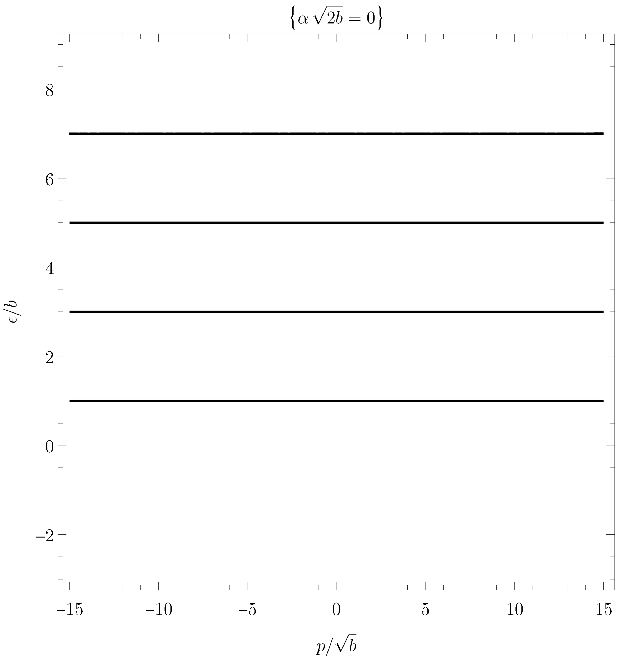
\includegraphics[width=0.45\textwidth]{grafy/dirac0.pdf}%
    \hspace{0.1\textwidth}%
    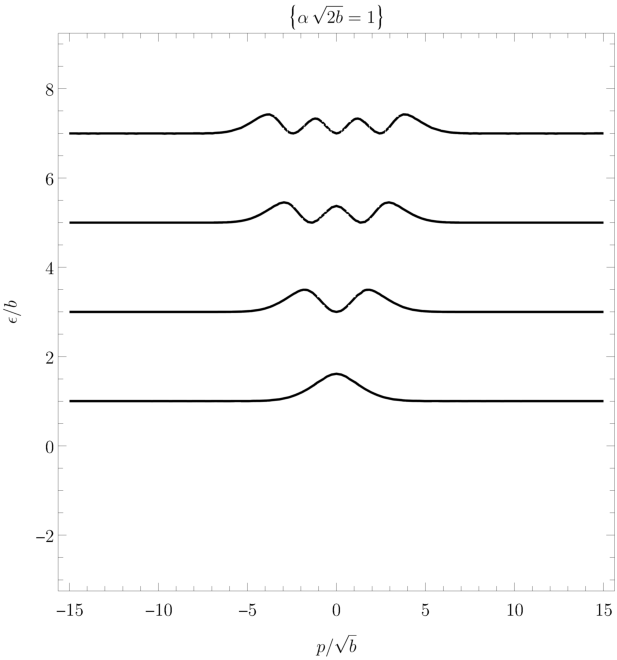
\includegraphics[width=0.45\textwidth]{grafy/dirac1.pdf}%
    \\[1em]%
    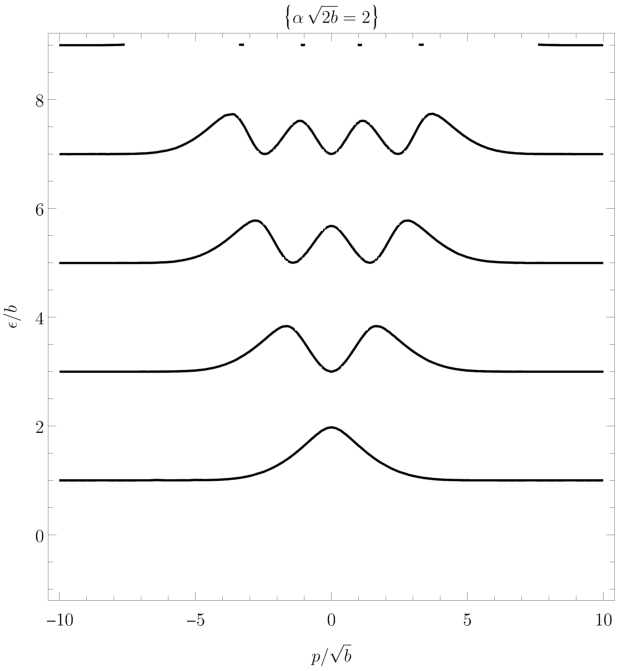
\includegraphics[width=0.45\textwidth]{grafy/dirac2.pdf}%
    \hspace{0.1\textwidth}%
    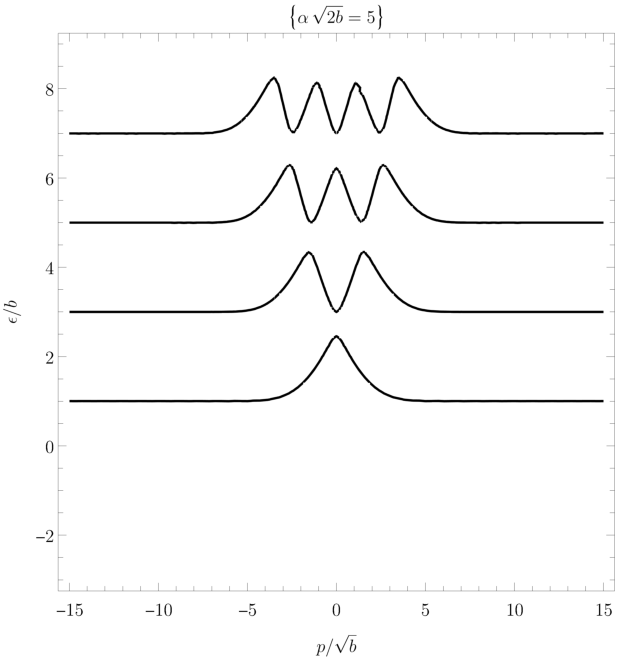
\includegraphics[width=0.45\textwidth]{grafy/dirac5.pdf}%
    \\[1em]%
    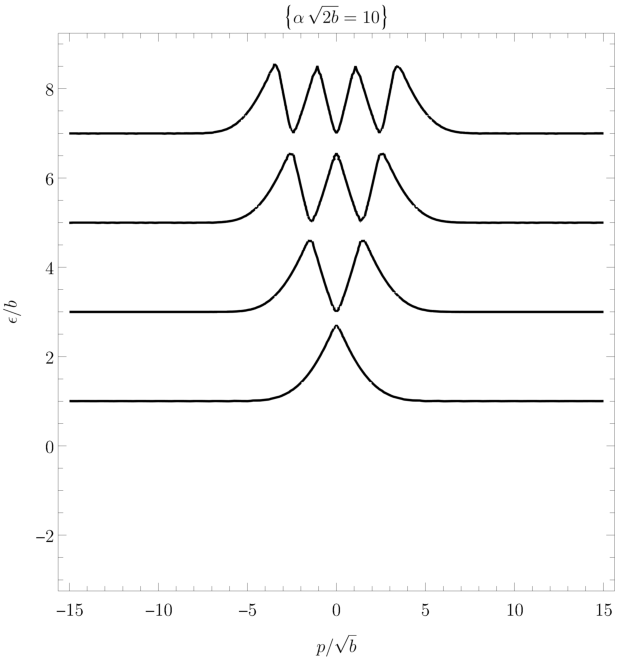
\includegraphics[width=0.45\textwidth]{grafy/dirac10.pdf}%
    \hspace{0.1\textwidth}%
    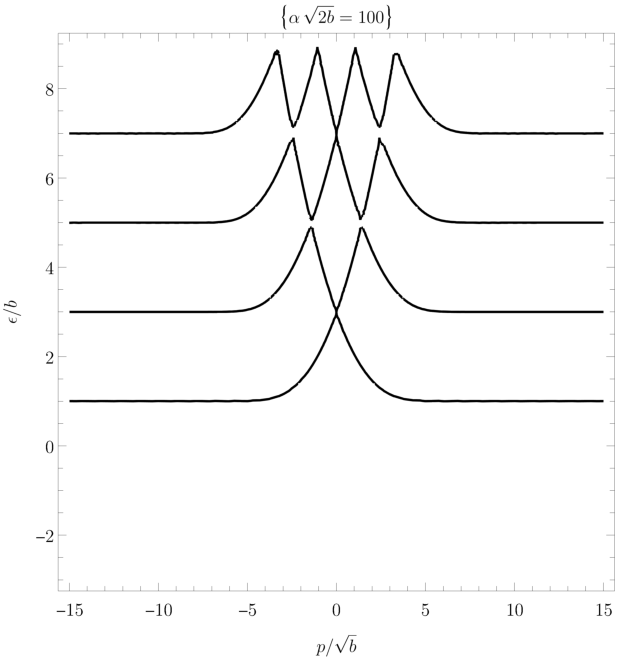
\includegraphics[width=0.45\textwidth]{grafy/dirac100.pdf}\par
    \caption{The first four energy levels $\epsilon$ as a function of the $y$-momentum $p$ for $\alpha\,\sqrt{2b} = 0, 1, 2, 5, 10$ and $100$ (starting with an unperturbed system, followed by an increasingly repulsive perturbation).}
    \label{plots-dirac-repulsive}
\end{figure}

\begin{figure}[p]
    \centering
    \noindent
    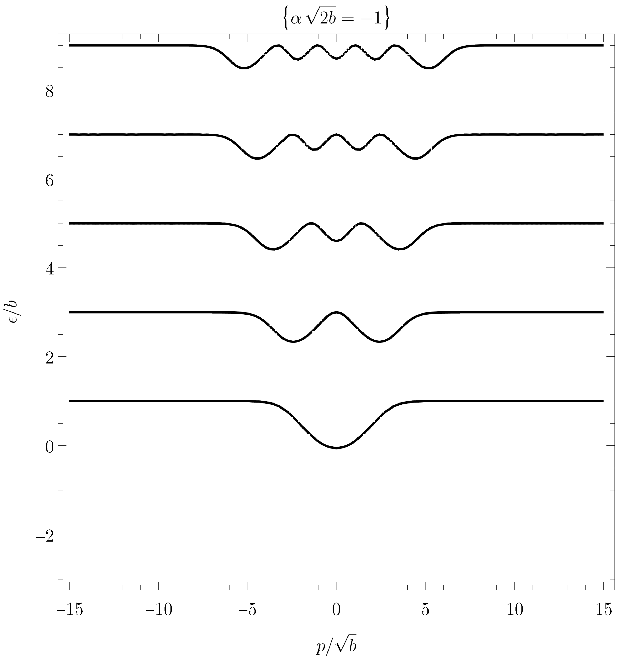
\includegraphics[width=0.45\textwidth]{grafy/dirac-1.pdf}%
    \hspace{0.1\textwidth}%
    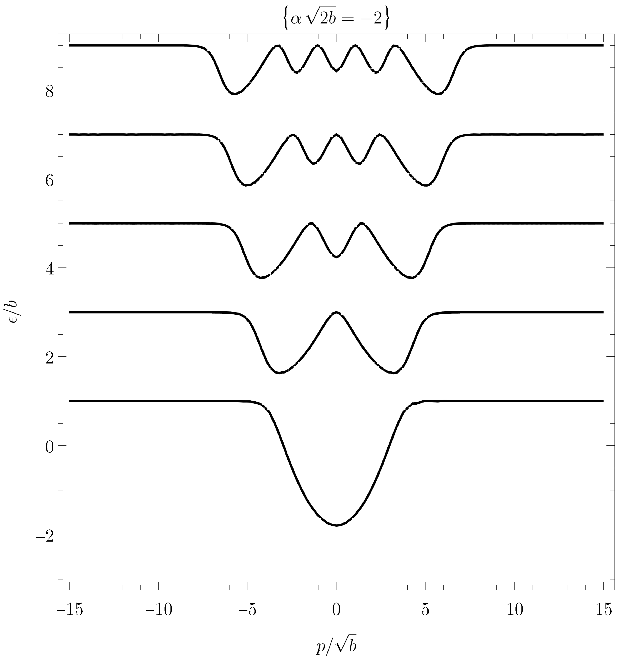
\includegraphics[width=0.45\textwidth]{grafy/dirac-2.pdf}%
    \\[2em]%
    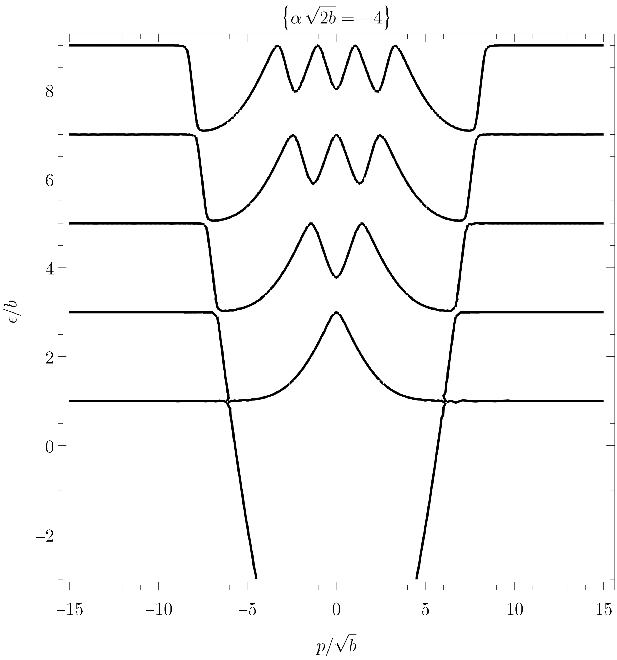
\includegraphics[width=0.45\textwidth]{grafy/dirac-4.pdf}%
    \hspace{0.1\textwidth}%
    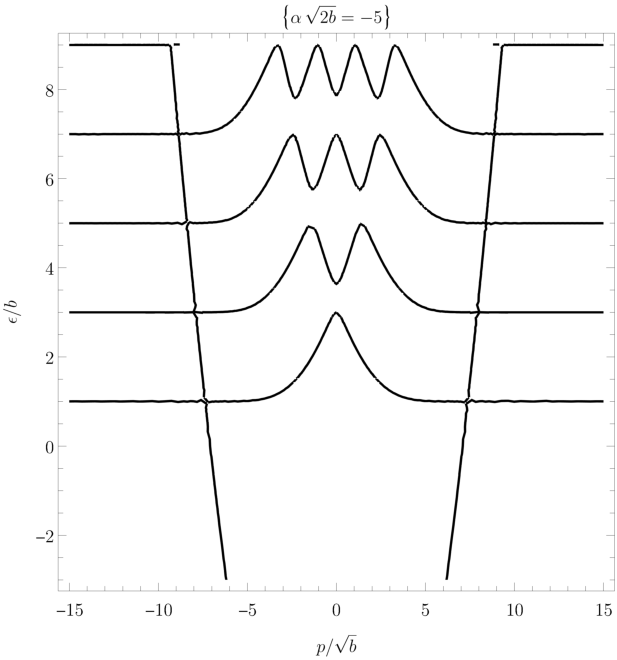
\includegraphics[width=0.45\textwidth]{grafy/dirac-5.pdf}\par
    \caption{The first five energy levels $\epsilon$ as a function of the $y$-momentum $p$ for $\alpha\,\sqrt{2b} = -1, -2, -4$ and $-5$ (system with an increasingly attractive perturbation).}
    \label{plots-dirac-attractive}
\end{figure}



\chapter*{Conclusion}
\addcontentsline{toc}{chapter}{Conclusion}

This thesis aimed to summarize the current knowledge of translationally invariant magnetic Hamiltonians and complement that knowledge with two previously unstudied systems.

One of the systems that we studied was the Landau Hamiltonian with a Dirac delta-interaction of strength $\alpha$ supported on a line. We verified that the Hamiltonian is self-adjoint and bounded from below, that it is a fibred operator and the spectrum of its fibre is discrete and nondegenerate. Then we found implicit expressions for the eigenvalues and eigenfunctions of the fibre Hamiltonian. Finally, we proved that: for a repulsive interaction ($\alpha>0$), there are spectral bands that start on each Landau level and extend up, for an attractive interaction ($\alpha < 0$), the spectral bands start on each Landau level and extend down. In both cases, the spectral bands never merge – there is a forbidden energy gap between each two neighbouring Landau levels. The spectrum of the Hamiltonian is absolute continuous; its singular continuous and pure point spectra are empty.

The other system that we examined was the Landau Hamiltonian on a half-plane with a Robin boundary condition. As with the delta-interaction, we verified the self-adjointness and boundedness from below, and that the fibre Hamiltonian has a discrete nondegenerate spectrum. Then we used the properties of the fibre to prove that: the spectrum of the Hamiltonian is absolute continuous, starting from a minimum below the first Landau level and extending up ad infinitum. We have numerically calculated estimates of the minimum energy for different values of the boundary parameter $\alpha$.

By comparing the (numerically computed) eigenvalues of the two systems' fibre Hamiltonians, we observed that if $p_y \ll 0$ and $|\alpha|$ is large enough, then the energy levels of the Robin-boundary fibre Hamiltonian with parameter $\alpha$ are a good approximation of the fibre Hamiltonian of a $\delta$-interaction of strength $-\alpha$.

Topics for further studies on the spectral properties of translationally invariant magnetic Hamiltonians are far from exceeded. Regarding the two Hamiltonians we studied, future work might investigate the stability of their spectra under perturbations by various classes of disorder potentials, or find upper and lower estimates for the minimum energy of the Robin half-plane Hamiltonian. Other Landau Hamiltonians with potential perturbations which, to the author's knowledge, are yet to be studied include: multiple $\delta$-interactions on parallel lines, a $\delta'$-interaction\footnote{The plausibility of a $\delta'$-interaction in one dimension is discussed in Chapter III.3 of \cite{Albeverio2005}.} supported on a line or multiple parallel lines, and a strip with Neumann or Robin boundaries.


%%% Bibliography
%%% Bibliography (literature used as a source)
%%%
%%% We employ bibTeX to construct the bibliography. It processes
%%% citations in the text (e.g., the \cite{...} macro) and looks up
%%% relevant entries in the bibliography.bib file.
%%%
%%% The \bibliographystyle command selects, which style will be used
%%% for references from the text. The argument in curly brackets is
%%% the name of the corresponding style file (*.bst). Both styles
%%% mentioned in this template are included in LaTeX distributions.

\bibliographystyle{plainnat}    %% Author (year)
% \bibliographystyle{unsrt}     %% [number]

\renewcommand{\bibname}{Bibliography}

%%% Generate the bibliography. Beware that if you cited no works,
%%% the empty list will be omitted completely.

\bibliography{bibliography}

%%% If case you prefer to write the bibliography manually (without bibTeX),
%%% you can use the following. Please follow the ISO 690 standard and
%%% citation conventions of your field of research.

% \begin{thebibliography}{99}
%
% \bibitem{lamport94}
%   {\sc Lamport,} Leslie.
%   \emph{\LaTeX: A Document Preparation System}.
%   2nd edition.
%   Massachusetts: Addison Wesley, 1994.
%   ISBN 0-201-52983-1.
%
% \end{thebibliography}


%%% Figures used in the thesis (consider if this is needed)
\listoffigures

%%% Tables used in the thesis (consider if this is needed)
%%% In mathematical theses, it could be better to move the list of tables to the beginning of the thesis.
\listoftables

%%% Abbreviations used in the thesis, if any, including their explanation
%%% In mathematical theses, it could be better to move the list of abbreviations to the beginning of the thesis.
% \chapwithtoc{List of Abbreviations}

%%% Attachments to the bachelor thesis, if any. Each attachment must be
%%% referred to at least once from the text of the thesis. Attachments
%%% are numbered.
%%%
%%% The printed version should preferably contain attachments, which can be
%%% read (additional tables and charts, supplementary text, examples of
%%% program output, etc.). The electronic version is more suited for attachments
%%% which will likely be used in an electronic form rather than read (program
%%% source code, data files, interactive charts, etc.). Electronic attachments
%%% should be uploaded to SIS and optionally also included in the thesis on a~CD/DVD.
%%% Allowed file formats are specified in provision of the rector no. 72/2017.
\appendix
\chapter{Appendix}
\section{Sobolev-type inequality}
\label{apdx-sobolev-ineq}

In this section we prove a Sobolev-type inequality analogical to the inequality (7.16) in \cite{BEH}. The presented proof is a simple modification of their proof.
\begin{lemma}
	Let $\psi \in W^{1,2}(\R)$, then for every $a>0$ there exists $b>0$ such that
	\begin{equation}
		\norm{\psi}^{\,n}_{L^\infty(\R)}
		\leq
		a \, \norm{\psi'}^{\,n}_{L^2(\R)} +
		b \, \norm{\psi}^{\,n}_{L^2(\R)}
		\: ,
		\label{sobolev-type-0}
	\end{equation}
	where $n \in \{ 1, 2 \}$.
	\label{lemma-sobolev-type-inequality}
\end{lemma}
\begin{proof}
	We define $\phi := \Fourier \psi$. Since, by definition, $\psi' \in L^2(\R)$ we have $\Fourier \psi' = T_x \Fourier \psi = T_x \phi \in L^2(\R)$, where $T_x$ means the operator of multiplication by the identity function $x \mapsto x$. Next, we utilize the Hölder inequality to find an estimate of $\lVert\phi\rVert_{L^1}$.
	\begin{equation}
		\norm{\phi}_{L^1}
		\!=
		\norm{\tfrac{1}{x+\i} \, (x+\i) \, \phi(x) }_{L^1}
		\!\leq \underbrace{ \norm{\tfrac{1}{x+\i}}_{L^2} }_{=: \, c}
		\; \norm{(x+\i) \, \phi(x)}_{L^2}
		\leq \,c\, \Big(
			\norm{T_x \, \phi}_{L^2} \!+
			\norm{\phi}_{L^2}
		\Big)
		\: .
		\label{sobolev-type-1}
	\end{equation}
	Since $\phi \in L^1$, it follows that $\psi \in L^\infty$ and
	\begin{equation}
		\norm{\psi}_{L^\infty}
		\leq \frac{1}{\sqrt{2\pi}} \,
		\norm{\phi}_{L^1}
		\: .
		\label{sobolev-type-2}
	\end{equation}
	We introduce a scaled function $\phi_r(x) := r \, \phi(r x)$. Scaling changes the norms in the following way:
	\begin{gather*}
		\norm{\phi_r}_{L^2}^{\,2}
		= r \, \norm{\phi}_{L^2}^{\,2}
		\: ,
		\qquad
		\norm{T_x \phi_r}_{L^2}^{\,2}
		= \frac{1}{r} \, \norm{T_x}_{L^2}^{\,2}
		\: .
	\end{gather*}
	By substituting $\phi \mapsto \phi_r$ in \eqref{sobolev-type-1} and combining with \eqref{sobolev-type-2}, we get
	\begin{gather*}
		\norm{\psi}_{L^\infty}
		\leq
		c \, \sqrt{r} \, \norm{T_x \, \phi}_{L^2} \!+
		\frac{c}{\sqrt{r}} \, \norm{\phi}_{L^2}
		=
		c \, \sqrt{r} \, \norm{\psi'}_{L^2} \!+
		\frac{c}{\sqrt{r}} \, \norm{\psi}_{L^2}
		\: .
	\end{gather*}
	Choosing $r = a^2/c^2$, we have proven the inequality \eqref{sobolev-type-0} for $n=1$.
	\\{}[\textbf{Dodělat $n=2$ podle BEH nerovnost (4.3) a diskuse pod ní.}]
\end{proof}


\openright
\end{document}
